\documentclass[notitlepage]{report}
\usepackage[left=1in, right=1in, top=1in, bottom=1in]{geometry}

%Para usar colores en las tablas:
\usepackage{color}
%\usepackage{graphicx} DUPLICADO
\usepackage{epsfig}
\usepackage{multirow}
\usepackage{colortbl}
\usepackage[table]{xcolor}
%Fin de pacquetes para usar colores en las tablas


\usepackage{titling}
\usepackage{lipsum}
\usepackage{mathtools}
\usepackage{amsmath}
\usepackage{amsfonts}
\usepackage{amssymb}
\usepackage{pdfpages}
\usepackage[spanish]{babel}
\usepackage[utf8]{inputenc}
\setlength{\parskip}{2mm}
\usepackage{graphicx}
\graphicspath{ {../Imagenes/Editadas/} } 

%Definiendo colores:
\definecolor{lightgray}{gray}{0.9}
\definecolor{myblue}{RGB}{180,241,231}
\definecolor{myred}{RGB}{241,121,108}
\definecolor{myyellow}{RGB}{245,239,122}
%Fin de definicion de colores:


\pretitle{\begin{center}\Huge\bfseries}
	\posttitle{\par\end{center}\vskip 0.5em}
\preauthor{\begin{center}\Large\ttfamily}
	\postauthor{\end{center}}
\predate{\par\large\centering}
\postdate{\par}

\title{Diagonalización Inversa} 
\author{Juan Carlos Caso Alonso y Francisco Mario Cruz Almeida}
\date{\today}


\begin{document}
	
	\maketitle
	\thispagestyle{empty}
	
	\newpage
\renewcommand{\abstractname}{Abstract}
\begin{abstract}
	
	Testar la veracidad del Teorema de Cantor, no debería llevarnos a ningún lado excepto comprobar su solidez. Digamos que en el viaje realizado, buscando formas de ponerlo a prueba, me he encontrado una serie de fenómenos numéricos. 
	
	
	Algunos son solo redescubrimientos de cosas conocidas. Otros son cosas interesantes, aparentemente nuevas, pero sin demasiada relevancia en el campo de la teoría de conjuntos. Por ejemplo: haber encontrado un patrón común entre diversas biyecciones famosas, creando alternativas al uso de números primos.
	
	
	Pero hay dos fenómenos numéricos bastante curiosos. Por separado, sobre cada uno de ellos, han opinado dos matemáticos diferentes sin conocer la existencia del otro fenómeno. Lo curioso es que las contra-argumentaciones de ambos, se vuelven contradictorias, cuando mezclamos ambos fenómenos en uno: un intento de diagonalización inversa. La contra-argumentación de uno, le quita la razón al otro y viceversa.
	
	
	Un proceso, la diagonalización inversa, por el cual intentaremos 'afirmar' una consecuencia cardinal entre un conjunto, LCF, con el mismo cardinal que $\mathbb{N}$ y otro conjunto, SNEIs, con el mismo cardinal que $P(\mathbb{N})$. La novedad es que invertiremos los papeles: partiremos de afirmar que SNEIs tiene un cardinal mayor que LCF, y para que eso suceda, debe ser 'posible' hallar una 'muestra', muy concreta, de esa diferencia cardinal. La gracia va a estar en que nos va a resultar totalmente imposible hallarla. Y para 'mostrarlo', dada la singularidad del caso, podremos usar argumentos tremendamente similares a los de la diagonalización.
	
	
	Al final vamos a obtener un fenómeno con las mismas fortalezas y debilidades que dos técnicas de diagonalización usadas por Cantor. Y uso el término 'debilidades', pues las contra-argumentaciones a este fenómeno tienen 'traducción' directa en las diagonalizaciones cantorianas, donde no se consideran 'debilidades'. Las similitudes van a ser tremendamente asombrosas.
	
	
	Por eso, este documento consistirá en la exposición de varios fenómenos numéricos, y de explicar como funcionan en equipo para crear la susodicha diagonalización inversa.
	
	
	A pesar de usar definiciones correctas, siempre comienzan diciéndome que son confusas, para acabar aceptando su validez. Simplemente por su densidad inicial. No siendo, las definiciones, totalmente formales, se entienden rápida y perfectamente. No hay forma de acelerar o suavizar el viaje, así que tendremos que ir con calma, explicando y definiendo los conceptos del contexto de dichos fenómenos. Va a ser triste, por la simpleza de muchos de ellos... pero la experiencia me indica que es un viaje inevitable. Juro que las mismas personas han pasado de decir cosas como 'ininteligible' o 'confuso', a cosas como 'obvio' o 'trivial', simplemente por no haberlo leído bien, dado el tema que 'sobrevuela' a mi trabajo.
	
	
	Una vez expuestos, que cada cual les encuentre el sentido que desee. Pero su existencia es innegable.
			
\end{abstract}
		
	\addtocontents{toc}{\hspace{-7.5mm} \textbf{Capítulos}}
	\addtocontents{toc}{\hfill \textbf{P\'agina} \par}
	\addtocontents{toc}{\vspace{-2mm} \hspace{-7.5mm} \hrule \par}
	
	\tableofcontents
		
	\chapter{Introducción}

PROBANDO CAMBIOS

\begin{figure}[h!]
	%width=\textwidth
	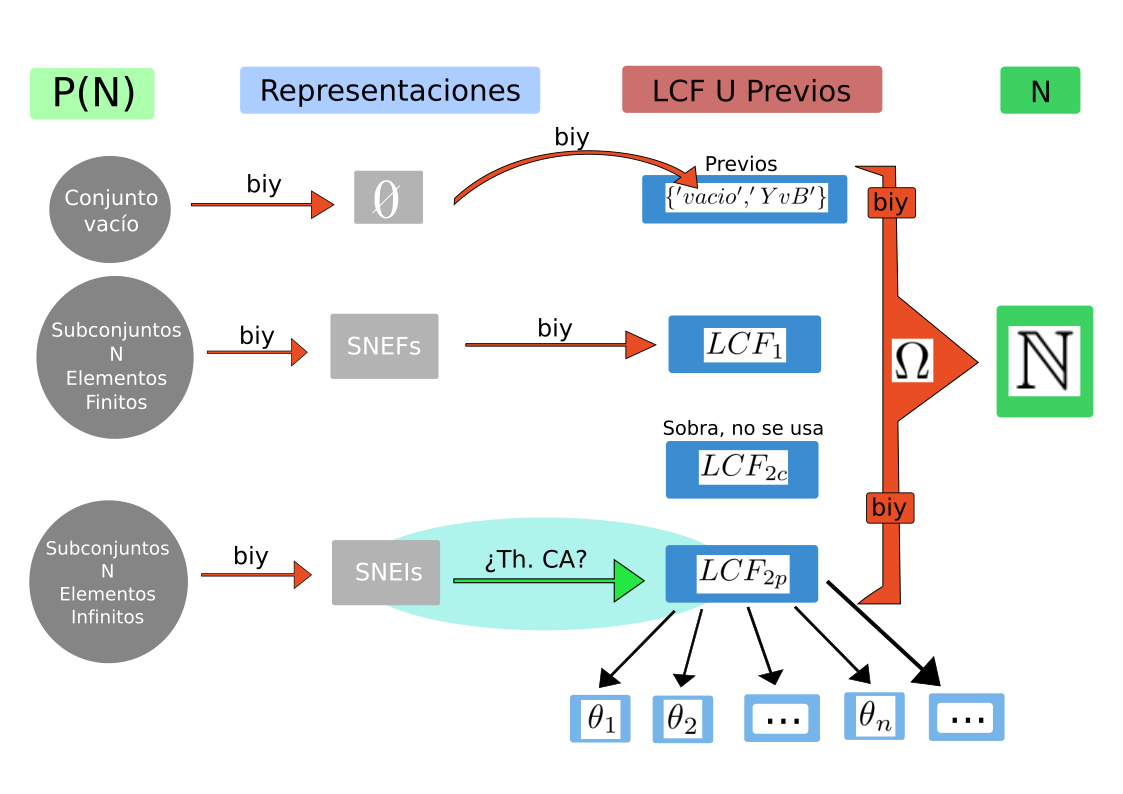
\includegraphics[ scale=0.7, angle=90]{EsquemaRelaciones}
	%\includegraphics[width=\textwidth, scale=0.3]{Funcion_hx_002_v4}
	%\includegraphics[width=\textwidth, scale=0.3]{Funcion_hx_001_v4}
	\centering
\end{figure}

\end{document}